\subsection{Nov\v cana naknada}

Nezaposleno lice dolazi u Nacionalnu slu\v zbu za zapo\v sljavanje radi ostvarivanja prava na nov\v canu naknadu. Kako bi nezaposleno lice ostvarilo pravo na nov\v canu naknadu ono mora da se prvo prijavi za ostvarivanje iste.
\\
Nakon \v sto se prijavi za ostvarivanje prava na nov\v canu naknadu, nezaposleno lice ide kod upravnog referenta da mu preda potrebnu dokumentaciju.
\\ Predata dokumenta prosle\dj uju se zajedno sa prijavom pravnom licu koje na osnovu zakonskih odredbi i prilo\v zene dokumentacije odlu\v cuje da li je nezaposleno lice ostvarilo pravo na nov\v canu naknadu ili nije.
\\
Odluka se prosle\dj uje kod direktora na overu i zatim u pisarnicu odakle se \v salje po\v stom nezaposlenom licu.

\subsubsection{Slu\v caj upotrebe: Prijava za ostvarivanja prava na nov\v canu naknadu}
\label{su: prijava}
\noindent U\v cesnici: Nezaposleno lice (u daljem tekstu NL), \v Salterski slu\v zbenik (u daljem tekstu \v SS)
\\
\\ Preduslovi: NL ima li\v cnu kartu.
\\
\\ Postuslovi: Prijava je popunjena i prosle\dj ena upravnom referentu.
\\
\\ Glavni tok:
\begin{enumerate}
\item NL prilazi automatu i bira opciju ''Prijava za nov\v canu naknadu''.
\item Automat bele\v zi da je opcija ''Prijava za nov\v canu naknadu'' odabrana, ra\v cuna naredni broj u redu \v cekanja za tu opciju, i \v stampa papir sa brojem.
\item NL uzima broj i \v ceka svoj red.
	\item Kada do\dj e na red, NL prilazi evidencionom pultu i zahteva od \v SS da ga prijavi za nov\v canu naknadu.
	\item \v SS otvara formular za prijavu.
	\item \v SS tra\v zi od NL da mu preda li\v cnu kartu.
	\item NL predaje li\v cnu kartu.
    \item \v SS pronalazi NL u sistemu.
	\item \v SS daje NL-u da popuni Zahtev za ostvarivanje prava na nov\v canu naknadu.
	\item NL popunjava Zahtev za ostvarivanje prava na nov\v canu naknadu, a zatim ga vra\v ca \v SS-u.
	\item \v SS vra\v ca li\v cnu kartu NL-u i upu\' cuje ga kod upravnog referenta.
	\item Prelazi se na slu\v caj upotrebe \ref{su: kompletiranje dokumentacije}.
\end{enumerate}

\begin{description}
	\item[A1. Nezaposleno lice nije prijavljeno na evidenciju] ~\\
	Ukoliko u koraku 8. Glavnog toka \v SS ne mo\v ze da na\dj e NL u sistemu, zaklju\v cuje da NL nije prijavljeno na evidenciju tr\v zi\v sta rada i prelazi se na slu\v caj upotrebe \ref{su: prva prijava}.
\end{description}

\subsubsection{Slu\v caj upotrebe: Kompletiranje dokumentacije}
\label{su: kompletiranje dokumentacije}

\noindent U\v cesnici: Nezaposleno lice (u daljem tekstu NL), Upravni referent (u daljem tekstu UR).
\\
\\ Preduslovi: NL je popunio Zahtev za ostvarivanje prava na nov\v canu naknadu.
\\
\\ Postuslovi: UR je kompletirao dokumentaciju i prosledio je pravnom licu.
\\
\\ Glavni tok:
\begin{enumerate}
\item NL dolazi kod UR-a u kancelariju i predaje mu Zahtev za ostvarivanje prava na nov\v canu naknadu.
\item UR pronalazi NL u sistemu i dopunjava zahtev podacima iz evidencije.
\item UR tra\v zi od NL-a da mu preda potrebnu dokumentaciju.
\item NL predaje UR-u potrebnu dokumentaciju.
\item UR preuzima dokumentaciju i zahtev i \v salje pravnom licu na tuma\v cenje.
\item Prelazi se na slu\v caj upotrebe \ref{su: resenje}.
\end{enumerate}

\subsubsection{Slu\v caj upotrebe: Dono\v senje re\v senja o nov\v canoj naknadi}
\label{su: resenje}

\noindent U\v cesnici: Pravno lice.
\\
\\ Preduslovi: Upravni referent je predao Zahtev za ostvarivanje prava na nov\v canu naknadu i potrebnu dokumentaciju nezaposlenog lica pravnom licu.
\\
\\ Postuslovi: Nezaposleno lice je ili dobilo pravo na nov\v canu naknadu ili je odbijeno.
\\
\\ Glavni tok:
\begin{enumerate}
\item Pravno lice prima Zahtev za ostvarivanje prava na nov\v canu naknadu i potrebnu dokumentaciju.
\item Pravno lice proverava da li je sve ispravno popunjeno.
\item \begin{enumerate}
\item Pravno lice tuma\v ci zakon i na osnovu zakona i potrebne dokumentacije odobrava nov\v canu naknadu nezaposlenom licu.
\item Pravno lice tuma\v ci zakon i na osnovu zakona i potrebne dokumentacije ne odobrava nov\v canu naknadu nezaposlenom licu.
\end{enumerate}
\item Pravno lice prosle\dj uje re\v senje o nov\v canoj naknadi direktoru na overu.
\item Prelazi se na slu\v caj upotrebe \ref{su: gde je pecat}.
\end{enumerate}

\begin{description}
\item [A1. Nezaposleno lice nije predalo svu potrebnu dokumentaciju] ~\\
	U koliko u koraku 2. Glavnog toka primeti da fali neophodna dokumentacija pismenim putem obave\v stava nezaposleno lice da donese upravnom referentu nedostaju\' cu dokumentaciju. Prelazi se na slu\v caj upotrebe \ref{su: kompletiranje dokumentacije}.
\end{description}


\subsubsection{Slu\v caj upotrebe: Zaklju\v civanje re\v senja}
\label{su: gde je pecat}

\noindent U\v cesnici: Direktor.
\\
\\ Preduslovi: Pravno lice je donelo re\v senje o nov\v canoj naknadi i predalo ga direktoru.
\\
\\ Postuslovi: Re\v senje o nov\v canoj naknadi je overeno.
\\
\\ Glavni tok:
\begin{enumerate}
\item Direktor preuzima re\v senje o nov\v canoj naknadi.
\item Direktor analizira re\v senje o nov\v canoj naknadi.
\item Direktor overava re\v senje o nov\v canoj naknadi i prosle\dj uje ga pisarnici.
\item Prelazi se na slu\v caj upotrebe \ref{su: pisarnica}.
\end{enumerate}


\subsubsection{Slu\v caj upotrebe: Slanje re\v senja o nov\v canoj naknadi nezaposlenom licu}
\label{su: pisarnica}

\noindent U\v cesnici: Referent prijema i ekspedicije po\v ste (u daljem tekstu RPEP).
\\
\\ Preduslovi: Direktor je overio re\v senje o nov\v canoj naknadi i prosledio ga pisarnici.
\\
\\ Postuslovi: Re\v senje o nov\v canoj naknadi je poslato nezaposlenom licu.
\\
\\ Glavni tok:
\begin{enumerate}
\item RPEP preuzima overeno re\v senje o nov\v canoj naknadi.
\item RPEP pakuje re\v senje u kovertu.
\item RPEP \v cita adresu nezaposlenog lica iz sistema.
\item RPEP \v salje overeno re\v senje o nov\v canoj naknadi na pro\v citanu adresu.
\end{enumerate}

\begin{mylandscape}
	\subsubsection{BPMN dijagrami}
	
	\begin{figure}[H]
		\centering
		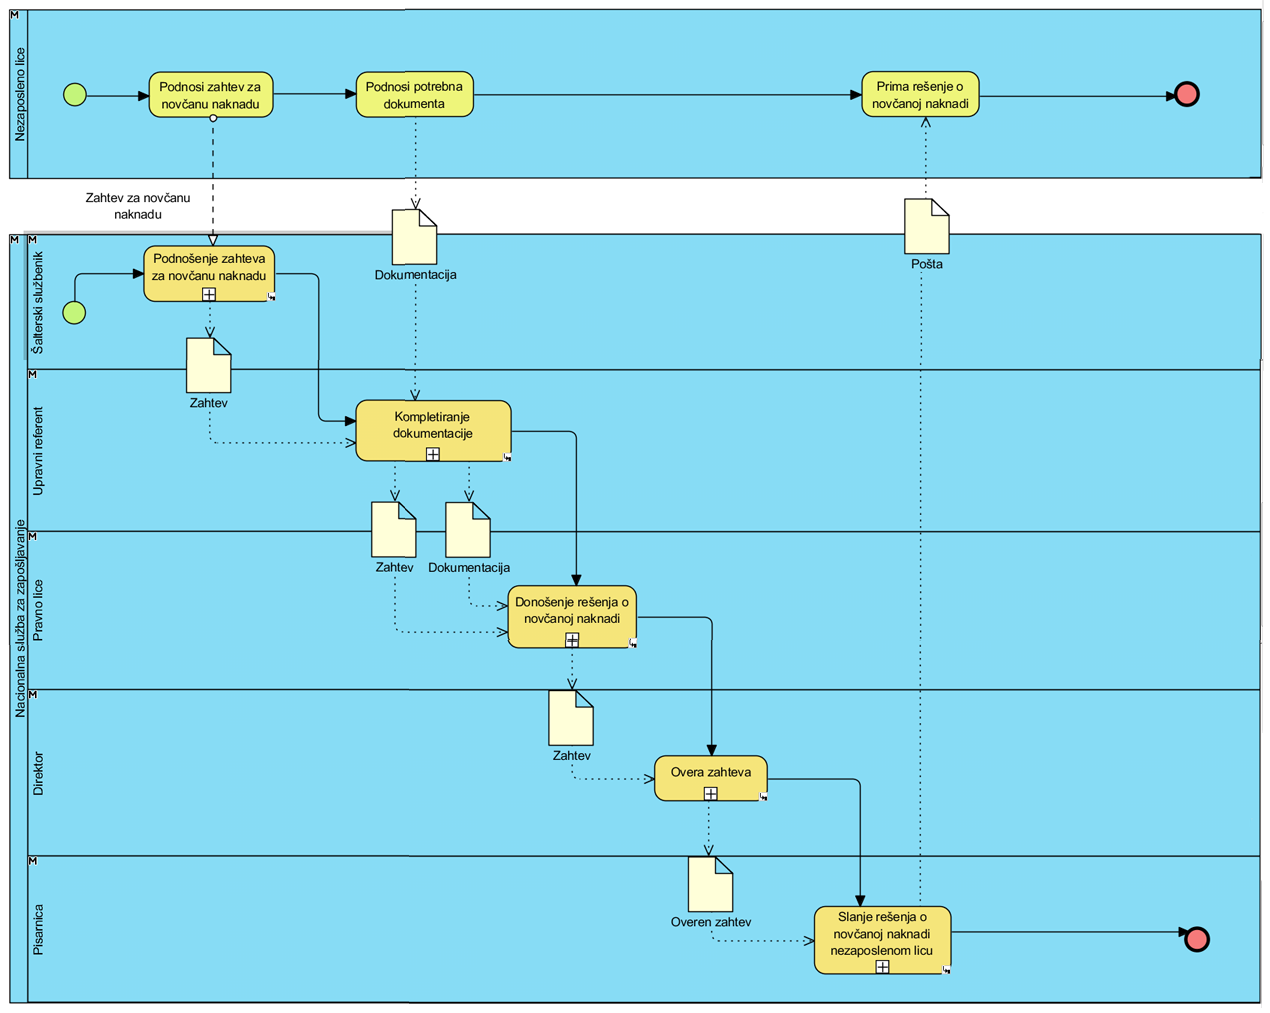
\includegraphics[width=0.6\paperwidth]{dijagrami/bpmn-dijagrami/bpmn-1.png}
		\caption{BPMN dijagram procesa ''Nov\v cana naknada''.}
		\label{bpmnd: novcana naknada}
	\end{figure}
	
	\newpage
	
	\begin{figure}[H]
		\centering
		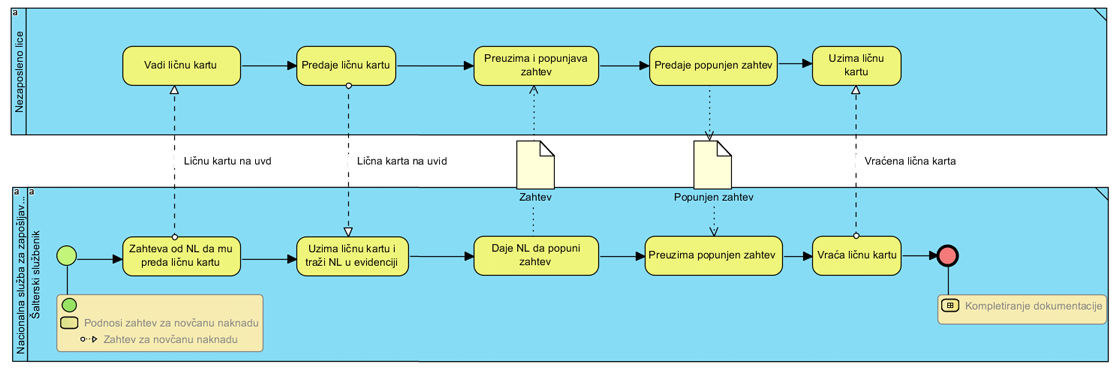
\includegraphics[width=0.6\paperwidth]{dijagrami/bpmn-dijagrami/bpmn-2.png}
		\caption{BPMN dijagram potprocesa ''Podno\v senje zahteva za nov\v canu naknadu'' procesa ''Nov\v cana naknada'' (\ref{bpmnd: novcana naknada}).}
	\end{figure}
	
	\begin{figure}[H]
		\centering
		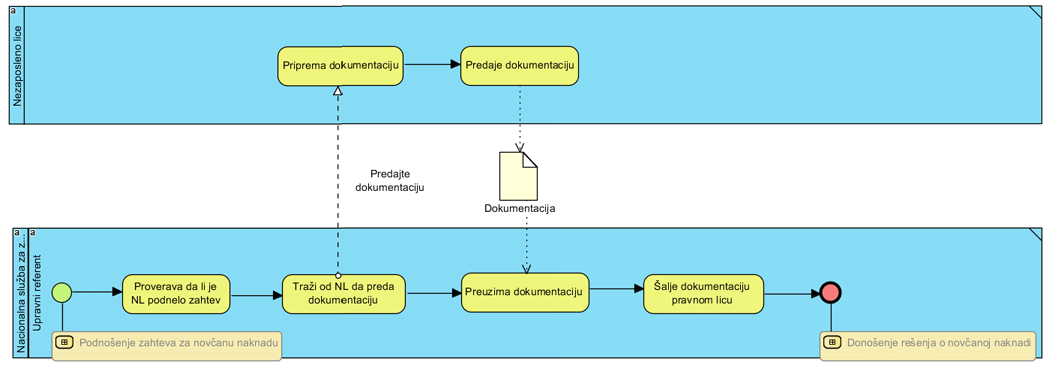
\includegraphics[width=0.6\paperwidth]{dijagrami/bpmn-dijagrami/bpmn-3.png}
		\caption{BPMN dijagram potprocesa ''Kompletiranje dokumentacije'' procesa ''Nov\v cana naknada'' (\ref{bpmnd: novcana naknada}).}
	\end{figure}

	\newpage
	
	\begin{figure}[H]
		\centering
		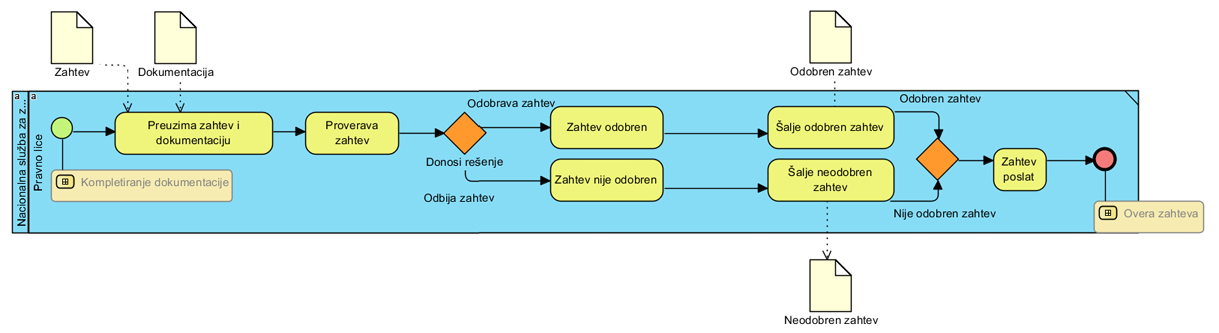
\includegraphics[width=0.6\paperwidth]{dijagrami/bpmn-dijagrami/bpmn-4.png}
		\caption{BPMN dijagram potprocesa ''Dono\v senje re\v senja o nov\v canoj naknadi'' procesa ''Nov\v cana naknada'' (\ref{bpmnd: novcana naknada}).}
	\end{figure}
	
	\begin{figure}[H]
		\centering
		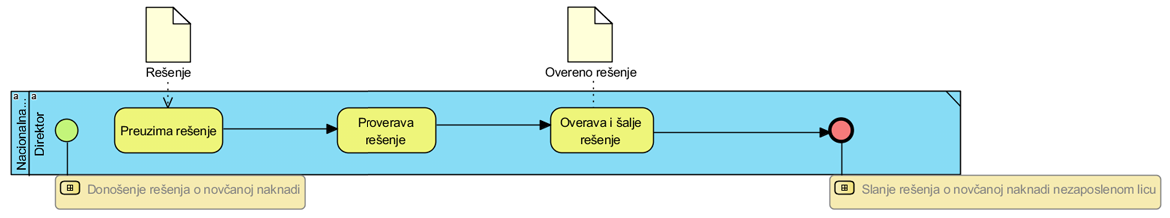
\includegraphics[width=0.6\paperwidth]{dijagrami/bpmn-dijagrami/bpmn-5.png}
		\caption{BPMN dijagram potprocesa ''Zaklju\v civanje re\v senja'' procesa ''Nov\v cana naknada'' (\ref{bpmnd: novcana naknada}).}
	\end{figure}

	\newpage
	
	\begin{figure}[H]
		\centering
		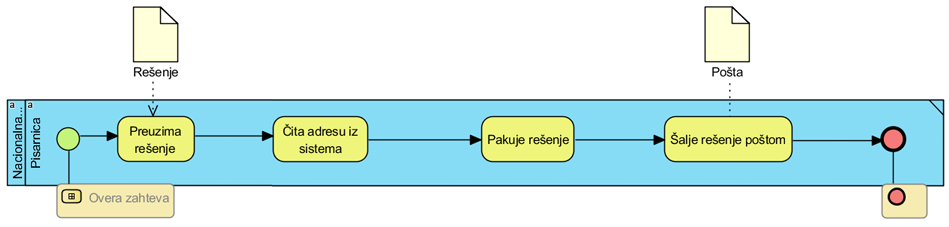
\includegraphics[width=0.6\paperwidth]{dijagrami/bpmn-dijagrami/bpmn-6.png}
		\caption{BPMN dijagram potprocesa ''Slanje re\v senja o nov\v canoj naknadi nezaposlenom licu'' procesa ''Nov\v cana naknada'' (\ref{bpmnd: novcana naknada}).}
	\end{figure}

\subsubsection{Dijagram stanja Zahteva za nov\v canu naknadu}
	\begin{figure}[H]
		\centering
		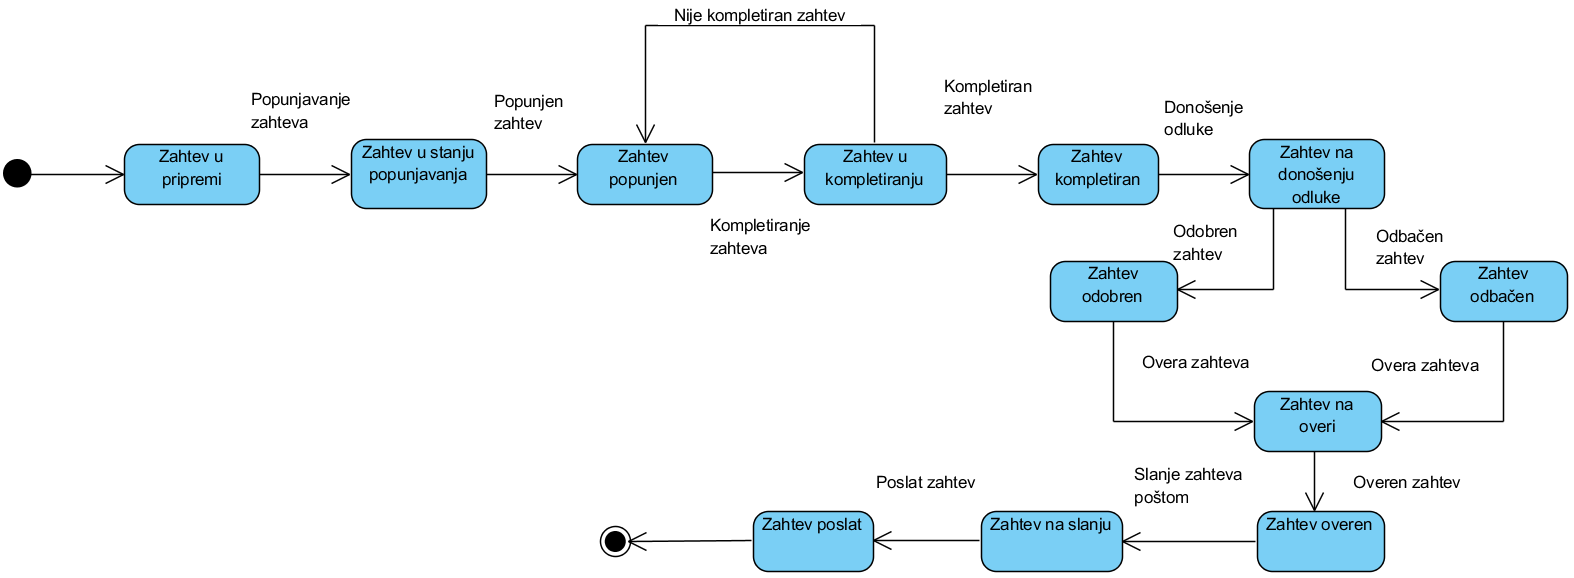
\includegraphics[width=0.6\paperwidth]{dijagrami/dijagrami-stanja/novcana-naknada.png}
		\caption{BPMN dijagram potprocesa ''Slanje re\v senja o nov\v canoj naknadi nezaposlenom licu'' procesa ''Nov\v cana naknada'' (\ref{bpmnd: novcana naknada}).}
	\end{figure}
	
	
\end{mylandscape}

